% DO NOT COMPILE THIS FILE DIRECTLY!
% This is included by the other .tex files.

\AtBeginSection[]
{
  \begin{frame}<beamer>{}
    %\tableofcontents[currentsection,currentsubsection]
    \tableofcontents[currentsection]
  \end{frame}
}

\begin{frame}[t,plain]
\titlepage
\end{frame}

\watermarkoff
%\begin{frame}[t]{Sommaire}
%\tableofcontents
%\end{frame}

\section{Bases du Libre}
\subsection{La Genèse}
\begin{frame}[t]{La Genèse}
    \begin{columns}
        \column{0.30\linewidth}
            \centering
                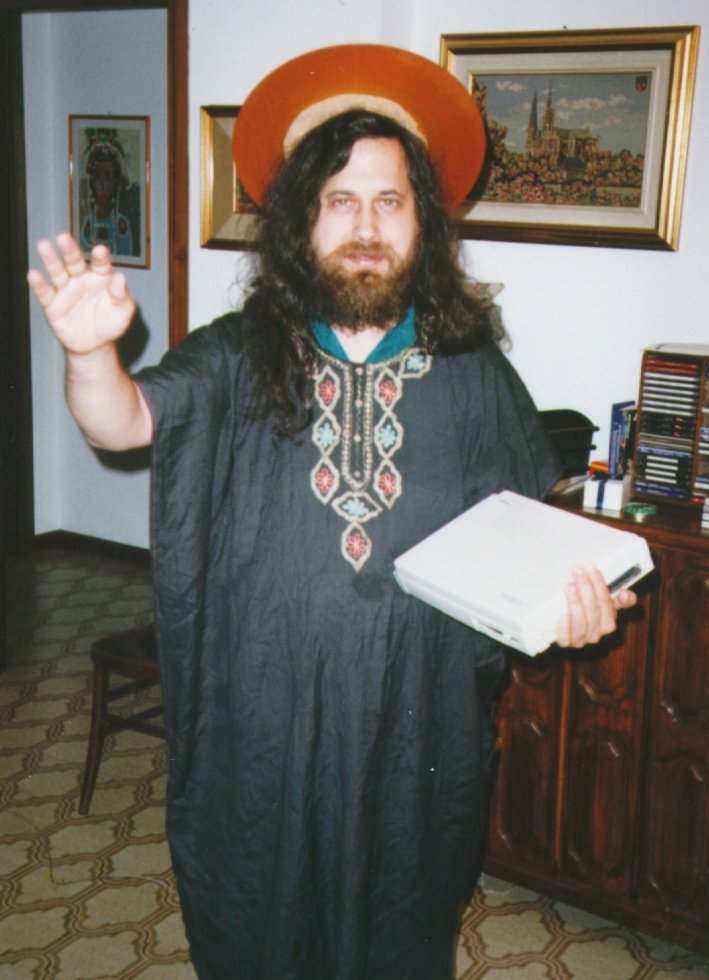
\includegraphics[height=5cm, width=3.5cm]{saintignucius}
        \column{0.70\linewidth}
            \begin{itemize}
                \item\fontsize{8}{10.5}\selectfont \textbf{Les bases du logiciel libre} ont été posées durant les années 80 par un certain Richard Stallman un programmeur qui milite pour de nombreuses cause : les logiciel libres, la neutralité et l’anonymat du web. \pause
               \item\fontsize{8}{10.5}\selectfont\textbf{Plutôt excentrique} il n'hésite pas à s’immiscer dans des locaux d’entreprises ou des bâtiments gouvernementaux afin d’exposer ses théories (refoulé de l’hotel Matignon).\pause
               \item\fontsize{8}{10.5}\selectfont\textbf{Il est le principal créateur} de la Free Software Foundation et l’instigateur du Projet GNU qui seront a l’origine de nombreux programmes dont certains seront très largement utilisés dans le monde, par exemple l'éditeur de texte Emacs et le compilateur GCC tous deux développés par Richard Stallman.
            \end{itemize}
    \end{columns}
\end{frame}

\subsection{Free Software Fondation}
\begin{frame}[t,fragile]{Free Software Foundation}
    \begin{columns}
    %\linebreak
    %\fontsize{10}{10.5}\selectfont
    \column{0.77\linewidth}
        \textbf{La Free Software Foundation} est une organisation à but non lucratif qui participe au financement et au développement du logiciel libre. \linebreak Cette fondation va être à l'origine des 4 libertés fondamentales de l'utilisateur :
         \column{0.23\linewidth}
    
\includegraphics[height=2.5cm, width=2.5cm]{logo_fsf} \pause
        \end{columns}
            \begin{itemize}
                \item \textbf{Liberté d’exécution} pour n'importe quel usage\pause
                \item \textbf{Liberté de modification personnelle}\linebreak ce qui nécessite la publication du code source.\pause
                \item \textbf{Liberté de redistribution} \pause
                 \item \textbf{Liberté de publication des version modifiées}
            \end{itemize}
\end{frame}


\begin{frame}[t,fragile]{Free Software Foundation}
    %\fontsize{8}{10.5}\selectfont  
     Cette fondation a également crée des licences logicielles pour protéger les logiciels libre. \pause
        \begin{itemize}
            \item \textbf{La licence GPL} (licence publique générale) : \pause
            \begin{itemize}
                \fontsize{9.5}{11}\selectfont
                \item[$\bullet$] \textbf{Utilisation libre} \pause
                \item[$\bullet$] \textbf {Code source public} \pause
                \item[$\bullet$] \textbf{Modifications autorisées}\linebreak mais doivent êtres publiés sous le \textbf{même type de licence}\linebreak (principe du Copyleft).\pause
                \item[$\bullet$] Il est impossible de récupérer des parties de code pour un logiciel propriétaire. \pause
            \end{itemize}
            \item \textbf{La licence LGPL} qui est identique a la licence GPL hormis le fait qu’il est possible de modifier le programme et de publier sous un autre type de licence.\pause
            \item \textbf{Attention un programme sous licence GPL/LGPL peut être payant.} 
        \end{itemize}
\end{frame}

\subsection{GNU}
\begin{frame}[t,fragile]{GNU}
    \fontsize{8}{10.5}\selectfont 
     \begin{columns}
        \column{0.30\linewidth}
            \centering
                
\includegraphics[height=5cm, width=3.5cm]{gerwinski-gnu-head}
        \column{0.70\linewidth}
        \textbf{GNU} est un projet visant à créer un système d’exploitation entièrement libre ainsi qu'une suite d’applications (libre office, the gimp ,konqueror) constituant une distribution.\linebreak Une avancée majeure dans ce projet fut la création par Linus Torvald en 1992 du Kernel Linux.\linebreak Ce noyau est une réécriture libre , inspirée du noyau propriétaire Unix, ces deux sont fréquemment confondus , c’est pour cela que l’acronyme GNU signifie Gnu is Not Unix.
    \end{columns}
\end{frame}

\begin{frame}[t,fragile]{GNU}
    \fontsize{9}{10.5}\selectfont
    Ce noyau va par la suite être très largement employé chez les développeurs et dans le domaine scientifique (super calculateurs), ainsi que dans l’armée (distribution legère basée sur un noyau linux plus securisé LPS). Mais n’arrivera pas à se démocratiser sur les PC de particuliers.\textbf{ Seulement 8\% des PC tournent sur OS basé sur linux (Mac OS compris)}, plusieurs raisons expliquent cela : \pause
    \begin{itemize}[<+->]
        \item[$\bullet$] \textbf{L’installation systématique de Windows} sur les ordinateurs vendus a conditionné les gens a son utilisation, rendant ainsi plus difficile le changement d’OS.%\pause
        \item[$\bullet$] \textbf{Les premières version des OS linux étaient peu “user friendly”}, et réputées pour être compliquées à maîtriser. %\pause
        \item[$\bullet$] Les fabriquants de matériel informatiques retissant à fournir des informations sur leurs produit ou adapter leurs pilotes sur les distributions Linux ou rendant son installation plus difficile.
    \end{itemize}
\end{frame}

\begin{frame}[t,fragile]{GNU}
    \fontsize{8}{10.5}\selectfont
        \begin{columns}
            \column{0.60\linewidth}
 Par exemple afin d’obtenir la certification Windows 8 les nouveaux ordinateurs devaient fournis un materiel utilisant \textbf{l’UEFI (BIOS graphique)} qui supporte la fonction \textbf{SecureBoot} permettant d'empêcher l'exécution de logiciels malveillant au démarrage de l’ordinateur grâce a un système de signature et de liste blanche. Cela a eu pour résultat la non possibilités d’installer les distributions Linux sur les ordinateurs ayant cette option activée.
            \column{0.40\linewidth}
                \centering
                    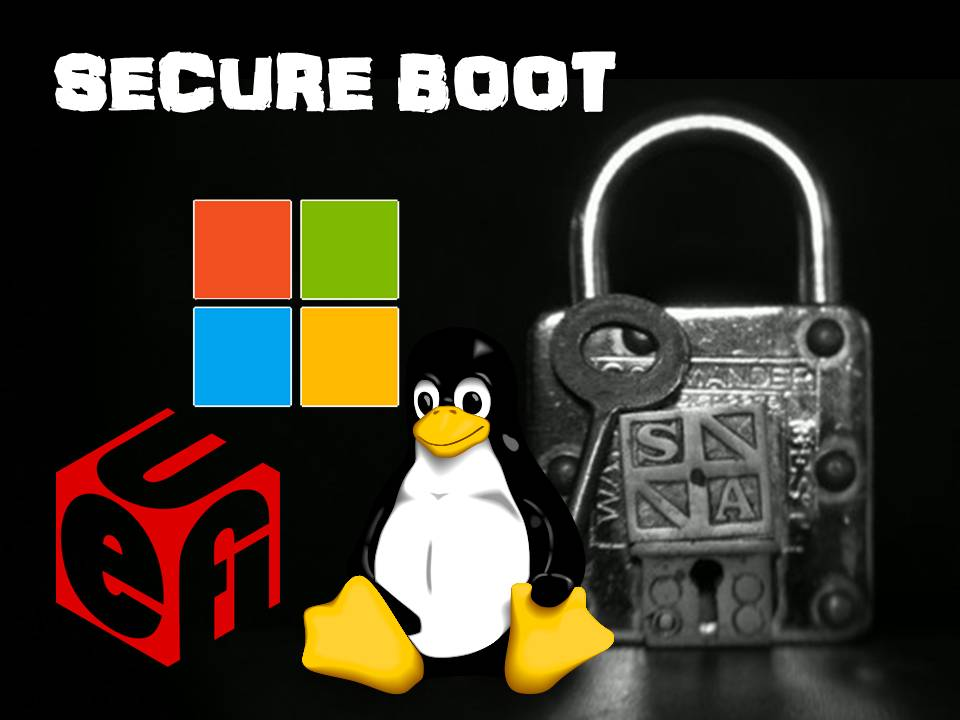
\includegraphics[height=5cm, width=4.5cm]{secure-boot}
        \end{columns}
\end{frame}

\begin{frame}[t,fragile]{GNU}
    \fontsize{8}{10.5}\selectfont
Actuellement, l’utilisation de distributions Linux augmente grace à Ubuntu. \linebreak Son utilisation est de plus en fréquente dans les entreprises, et les services publics principalement pour raison de coûts.
    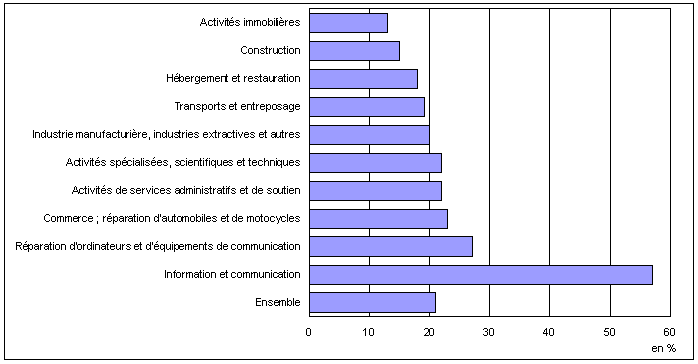
\includegraphics[height=4.75cm, width=11cm]{graphique1}
    \fontsize{8}{9}\selectfont \linebreak Répartition des OS libres dans les entreprises de plus de 10 salariés (INSEE)
\end{frame}


\subsection{Ubuntu}
\begin{frame}[t,fragile]{Ubuntu}
    \fontsize{8}{10}\selectfont
    \begin{columns}
        \column{0.70\linewidth}
                \textbf{Ubuntu} contrairement aux autres distributions est développé par une société: \textbf{Canonical Ltd.} \linebreak
Cette distribution n’est pas reconnue,comme beaucoup d’autres, par la FSF. Elle active par défaut l’utilisation de dépôts de paquets non libres et leur installation.
        \column{0.30\linewidth}
            \centering 
\includegraphics[height=2.5cm, width=3cm]{Canonical-logo}
    \end{columns} \pause
    \begin{columns}
        \column{0.40\linewidth}
            \centering 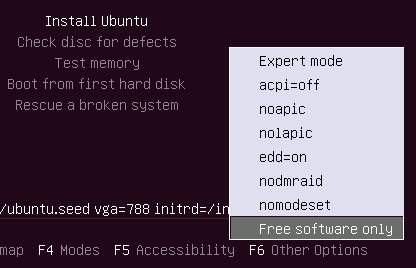
\includegraphics[height=4cm, width=5cm]{Ubuntu-foo}
        \column{0.60\linewidth}
            \textbf{Néanmoins cette option peut etre desactivée et ne conerne que très peu de paquets.}\linebreak \pause
            \centering 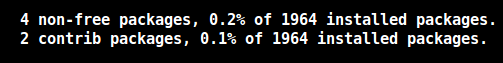
\includegraphics[height=1cm, width=7cm]{vrms}\linebreak Résultats de vrms sur Ubuntu 14.04.1
    \end{columns}
\end{frame}

\begin{frame}[t,fragile]{Ubuntu}
    \fontsize{9}{10}\selectfont
    La FSF ne soutient pas ubuntu principalement pour sa politique de développement qui privilégie "l'ergonomie" à la liberté de l'utilisateur.\linebreak \pause
        \begin{columns}
            \column{0.50\linewidth}
                \centering 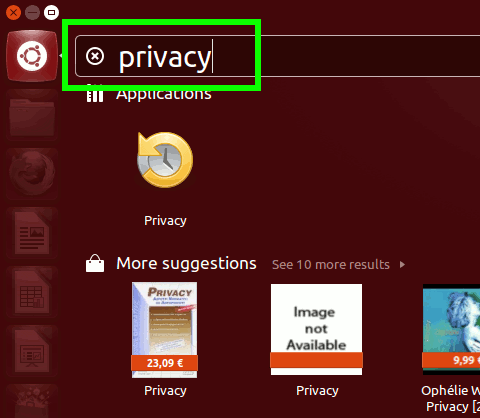
\includegraphics[height=4.5cm, width=6cm]{ubuntu-1210-dash}
            \column{0.50\linewidth}
    Par exemple, depuis la distribution 12.10, l'utilitaire de recherche dash comporte une partie recommandation amazon, orientée grâce aux termes de la recherche. \linebreak \pause
        \end{columns}
        \fontsize{9}{12}\selectfont
    Ce comportement n'est toléré par la FSF que si ce genre d'élément est \textbf{optionnel et très clairement expliqué} à l'utilisateur.
    
\end{frame}




\section{Open Source}
\subsection{Définition}
\begin{frame}[t,fragile]{Définition}
    \fontsize{8}{10.5}\selectfont
    \textbf{L’open source} crée par l’Open Source Initiative(OSI) désigne les logiciels dont le code doit être accessible et modifiable par tous librement, il ne faut donc pas le mélanger avec les logiciels propriétaires dit “open” dont le code source est accessible sous conditions.
On attribut a l’open source plusieurs avantages : \pause
    \begin{itemize}
        \item \textbf{la durée du support du programme} en effet n’importe qui peut reprendre le support du programme. \pause
        \item \textbf{la reduction des bogues} des qu’un bogue est détecté chaque membre de la communauté opensource peut le corriger \pause
        \item \textbf{la fiabilité} : la publication du code permet son analyse par la communauté et la correction d'éventuelles failles à condition que les membres participant au projet aient des notions de programmation avancées.\pause
        \item Mais la publication du code peut avoir l’effet inverse, car celui ci peut être étudié par des personnes mal intentionnées. En 2014, une faille sécurité majeure dans la solution de cryptage openSSL est découverte alors que celle ci était présente depuis 2012.
    \end{itemize}
\end{frame}

\subsection{Malentendus fréquents}
\begin{frame}[t,fragile]{Malentendus fréquents}
    \fontsize{10}{12}\selectfont
    \textbf{Il existe certaines différences} entre logiciel libre et logiciel open source.\pause
        \begin{itemize}
            \item La licence logiciel libre est plus restrictive en effet tous les \textbf{logiciels sous licence libre GNU/GPL sont open source mais l’inverse n’est pas forcement vrai.} \pause
            \item \textbf{Les notions de publication de code source est identique pour les 2 licences},\linebreak la différence entre les deux est plutôt d’ordre philosophique, en effet un logiciel “libre” est censé “respecter” les libertés de  l’utilisateur. \pause
            \item Si on prend l'exemple d'une application pouvant accepter des greffons (add-ons) mais obligeant l’utilisateur à les telecharger depuis son site uniquement.\linebreak \pause Cette application pourrait être open source mais pas libre car ne respectant pas la liberté de l’utilisateur.
        \end{itemize}
\end{frame}


\subsection{Licence Apache}
\begin{frame}[t,fragile]{Licence Apache}
    \fontsize{10}{12}\selectfont
    \begin{columns}
        \column{0.30\linewidth}
            \centering 
\includegraphics[height=2.5cm, width=3cm]{apache_feather}
        \column{0.70\linewidth}
            La licence Apache est une licence de logiciel libre approuvée par l'OSI crée par l'Apache Software Foundation(ASF).\pause
    \end{columns}
    \begin{itemize}
        \item[$\bullet$] Cette licence qui \textbf{n'est pas copyleft}, autorise la modification et la distribution du code sous toute forme\textbf{(libre ou propriétaire, gratuit ou commercial).}\pause 
        \item[$\bullet$] Elle assure le maintien du copyright lors de toute modification.\pause
        \item[$\bullet$] Elle peut être utilisée avec une licence GPLv3.
    \end{itemize}
\end{frame}

\subsection{Android}
\begin{frame}[t,fragile]{Android}
    \fontsize{8}{11}\selectfont
        \begin{columns}
            \column{0.30\linewidth}
                \centering 
\includegraphics[height=2.5cm, width=3cm]{android-logo}
            \column{0.70\linewidth}
    Le systeme d’exploitation mobile Android , developé par Google est composé du noyau Linux , et d’une machine virtuelle (Dalvik) permettant de lire du bytecode JAVA.\pause
        \end{columns}
        \begin{itemize}
            \item Ces deux programmes sont tous deux \textbf{distribués sous des licences différentes GPLv2 et Apache 2.0} une autre licence libre n'étant pas Copyleft, ces deux licences ne sont donc pas compatible. \pause
            \item Google doit publier le code source associé au noyau Linux et leurs modifications, \textbf{mais n’est pas obligé de publier ses modifications portés à la machine virtuelle}, car elles peuvent être placées sous licence propriétaire.\pause
            \item \textbf{Le code source publié serait donc incomplet et ne permettrait pas de faire fonctionner le systeme d’exploitation.}
    \end{itemize}
\end{frame}


\begin{frame}[t,fragile]{Android}
    \fontsize{9}{11}\selectfont
    \begin{itemize}
        \item Bien qu’il y ait eu plusieurs problèmes de publication de code avec Android 3.0, \textbf{l'intégralité du code est disponible faisant bien d’Android un logiciel libre.} \pause
        \item Malheureusement, bien qu’il soit libre, il est délibérément restreint matériellement par certains fabriquants, il est par exemple \textbf{impossible d’installer une version modifié du logiciel sur un appareil.} \pause 
        \item De plus dans la plupart des terminaux Android est \textbf{fourni avec de nombreuses applications propriétaire sans possibilités de desinstallation} (Android Market®). On se retrouve alors avec un logiciel “libre” occulté limitant les libertés de l’utilisateur.
    \end{itemize}
\end{frame}


\section{CONCLUSION}
\begin{frame}[t,fragile]{Compatibilités des licences libres}
    \centering 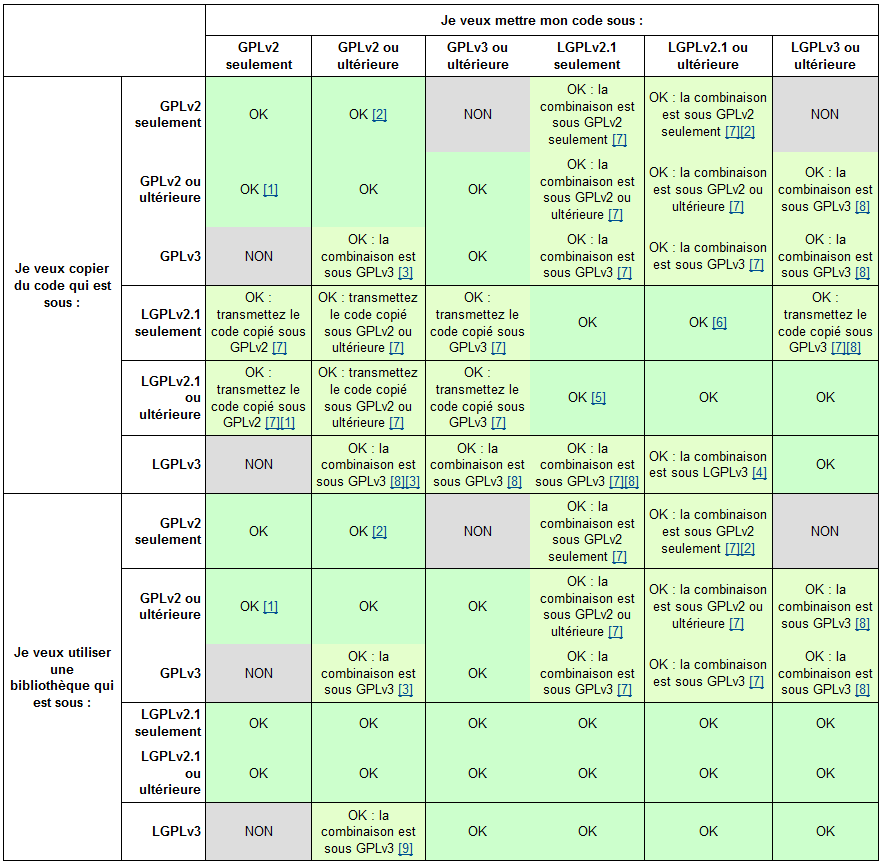
\includegraphics[height=7cm, width=11cm]{matrice_compat}
\end{frame}

\begin{frame}{Vue d'ensemble}
    \centering
        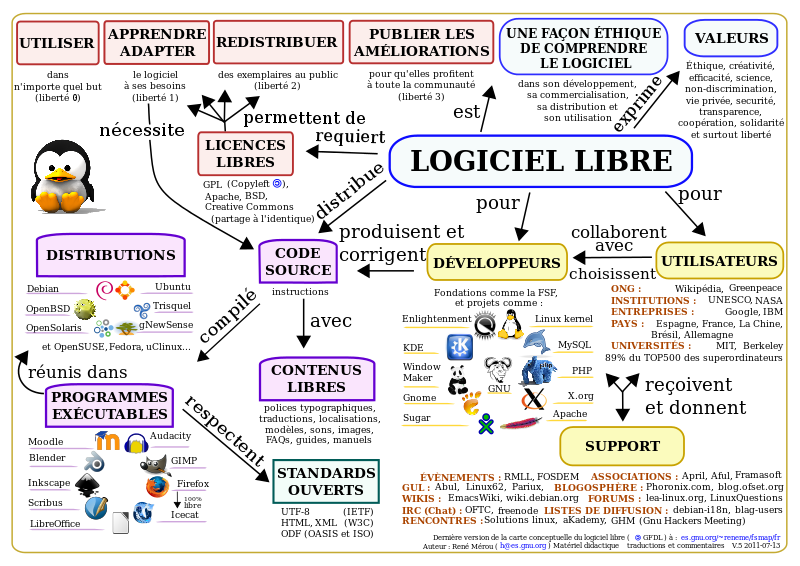
\includegraphics[height=7cm, width=11cm]{schema-logiciel-libre}
\end{frame}


